%%%%%%%%%%%%%%%%%%%%%%%%%%%%%%%%%%%%%%%%%
% University/School Laboratory Report
% LaTeX Template
% Version 3.1 (25/3/14)
%
% This template has been downloaded from:
% http://www.LaTeXTemplates.com
%
% Original author:
% Linux and Unix Users Group at Virginia Tech Wiki 
% (https://vtluug.org/wiki/Example_LaTeX_chem_lab_report)
%
% License:
% CC BY-NC-SA 3.0 (http://creativecommons.org/licenses/by-nc-sa/3.0/)
%
%%%%%%%%%%%%%%%%%%%%%%%%%%%%%%%%%%%%%%%%%

%----------------------------------------------------------------------------------------
%	PACKAGES AND DOCUMENT CONFIGURATIONS
%----------------------------------------------------------------------------------------

\documentclass{article}
\usepackage[spanish,es-tabla]{babel}

\usepackage[a4paper,
 %left=20mm,
 top=30mm,
 bottom=25mm,
 headheight=80pt,
 headsep=15mm
 ]{geometry}


\usepackage[version=3]{mhchem} % Package for chemical equation typesetting
\usepackage{graphicx} % Required for the inclusion of images

\usepackage{amsfonts}
\usepackage{amsmath} % Required for some math elements 
\usepackage{mathtools}

\usepackage{multirow}


\usepackage{changepage} % Required in text margins
\usepackage{xcolor} % Required changing color 
\usepackage{sectsty} %Required to change section headers
\usepackage{titlesec} % Required for section spacing
\usepackage{enumitem}
\usepackage{tocloft} % Better in table of contents
\usepackage[blocks]{authblk}% The option is for block layout
\usepackage[pdfborder={0 0 0}]{hyperref}% For email addresses
\usepackage{fancyhdr} %Required for Headers

\usepackage[nottoc]{tocbibind} %Better to add references and more in table of contents (nottoc is to remove indice in toc)

\usepackage{layout} %Used for "margin debugging"

\usepackage[export]{adjustbox} 
\usepackage{float}

\usepackage{subfig}% http://ctan.org/pkg/subfig


\pagestyle{fancy}
\fancyheadoffset{0cm} %Used for heading without margins
\fancyhead[L]{} % 1. sectionname

\rhead{ \textit{Simulaci\'on y Animaci\'on Biomec\'anica de un Humanoide}}
\renewcommand{\headrulewidth}{0.4pt}


\renewcommand\cfttoctitlefont{\hfill\huge\bfseries\color{cyan}}
\renewcommand\cftaftertoctitle{\hfill\mbox{}}

\setlist{leftmargin=5.5mm}

\titlespacing*{\section} {0pt}{6ex}{2ex}
\titlespacing*{\subsection} {0pt}{4ex}{0.7ex}

\sectionfont{\color{cyan}} % Changing color to section headers
\subsectionfont{\color{cyan}} % Changing color to subsection headers
\subsubsectionfont{\color{cyan}} % Changing color to subsubsection headers
\paragraphfont{\color{cyan}} % Changing color to subsubsubsection headers
%\setlength\parindent{0pt} % Removes all indentation from paragraphs

\renewcommand{\labelitemi}{$-$}

\renewcommand{\baselinestretch}{1.25} 

\usepackage{verbatimbox}
\newcommand{\at}{\makeatletter @\makeatother}

%----------------------------------------------------------------------------------------
%	DOCUMENT INFORMATION
%----------------------------------------------------------------------------------------

\begin{document}

\newpage


%(---------------------------------------------------------------------------------------
%	SECTION 1 - INTRODUCCION
%----------------------------------------------------------------------------------------


\section*{ Manual de Instalaci\'on - Proyecto Final Humanoide}

\begin{enumerate}
\item{ Clonar el repositorio \\
\textit{git clone git\at github.com:ealtamir/pf\_experimentos.git}
}

\item Crear una herramienta de l\'inea de comandos en XCode, seteando como lenguaje C++

\item Borrar el archivo $main.cpp$ en el proyecto antes creado

\item Arrastrar la carpeta $/code/src$ del proyecto y seleccionar la opci\'on ``Crear Grupos''

\item Arrastrar la carpeta $/code/include$ al proyecto y seleccionar la opci\'on ``Crear Grupos''

\item Mover el archivo $main.cpp$ de la carpeta $/code/src$ adonde estaba el archivo $main.cpp$ en el paso 3

\item Compilar las librer\'ias de bullet3 (https://github.com/bulletphysics/bullet3)
  
  [Install CMake](http://www.cmake.org/install/)

  Compilar las librer\'ias en OSX:
\textit{
     git clone git\at github.com:bulletphysics/bullet3.git\\
     cd bullet3\\
     cmake . -G ``Unix Makefiles'' -DINSTALL\_LIBS=ON -DBUILD\_SHARED\_LIBS=ON \\
      -DFRAMEWORK=ON  -DCMAKE\_OSX\_ARCHITECTURES='i386;x86\_64' \ \\
      -DCMAKE\_BUILD\_TYPE=RelWithDebInfo -DCMAKE\_INSTALL\_PREFIX=/Library/Frameworks \\
      -DCMAKE\_INSTALL\_NAME\_DIR=/Library/Frameworks -DBUILD\_DEMOS:BOOL=OFF\\
     make -j4 \\
     sudo make install
 }

\item Arrastrar las siguientes librer\'ias instaladas en la m\'aquina, en  $/Library/Frameworks/$ a la ra\'iz del proyecto:
    -BulletDynamics.framework\\
    -BulletCollision.framework\\
    -LinearMath.framework

\item Instalar galib:\\
        -Obtener el path a la carpeta $include$ de la librer\'ia GaLib, \\$\$REPOSITORY\_PATH/libraries/galib/247/include$\\
        -Ir a XCode, seleccionar el objetivo (o $target$) del proyecto y agregar ese path al ``Path de B\'usqueda del Header''\\
        -Tambi\'en agregar $libga.a$, arrastr\'andola a la ra'iz del proyecto en XCode ( $libga.a$ se encuentra en $\$REPOSITORY\_PATH/libraries/galib/247/lib/libga.a$).
       En caso de que la librer\'ia est\'atica no funcione, hacer lo siguiente: \textit{ brew install galib} 
        y encontrar el path donde est\'a instalado (generalmente ``/usr/local/Cellar/galib''). El \'arbol de la carpeta es como el descripto anteriormente para encontrar la librer\'ia est\'atica.

\item Arrastrar las librer\'ias est\'aticas en la carpeta $libraries$ en la carpeta ra\'iz del proyecto

\item Seleccionar la ra\'iz del proyecto, ir a ``Build phases'', abrir ``Link Binario con Librer\'ias'' y agregar:\\
    -GLUT.framework\\
    -OpenGL.framework\\

\item Seleccionar la ra\'iz del proyecto, ir a ``Build phases'', abrir ``C�digos de Compilaci\'on'' y agregar todos los archivos $.cpp$

Despu\'es de todo esto, se deber\'ia tener algo as\'i:
\begin{figure}[H]%
  \centering
  \frame{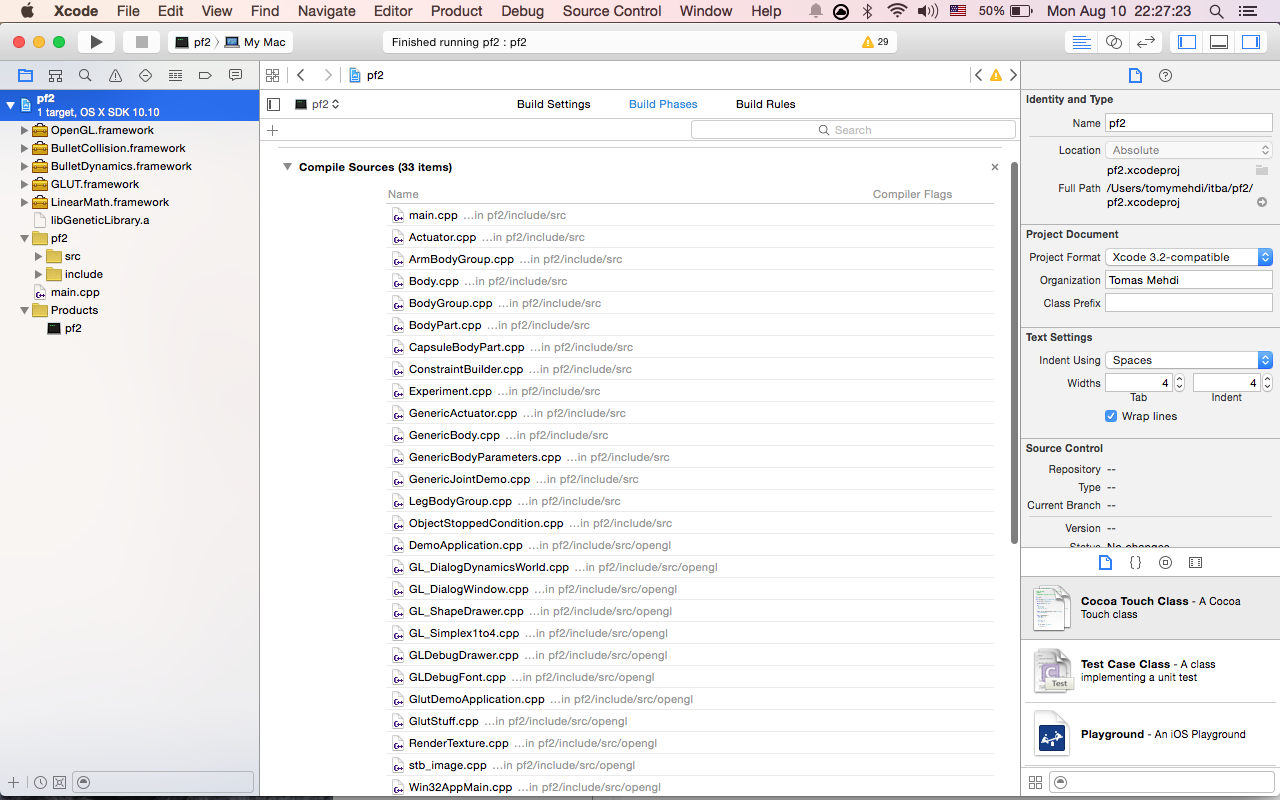
\includegraphics[width=0.72\linewidth]{readme1.png}} 
 \end{figure}

\begin{figure}[H]%
  \centering
  \frame{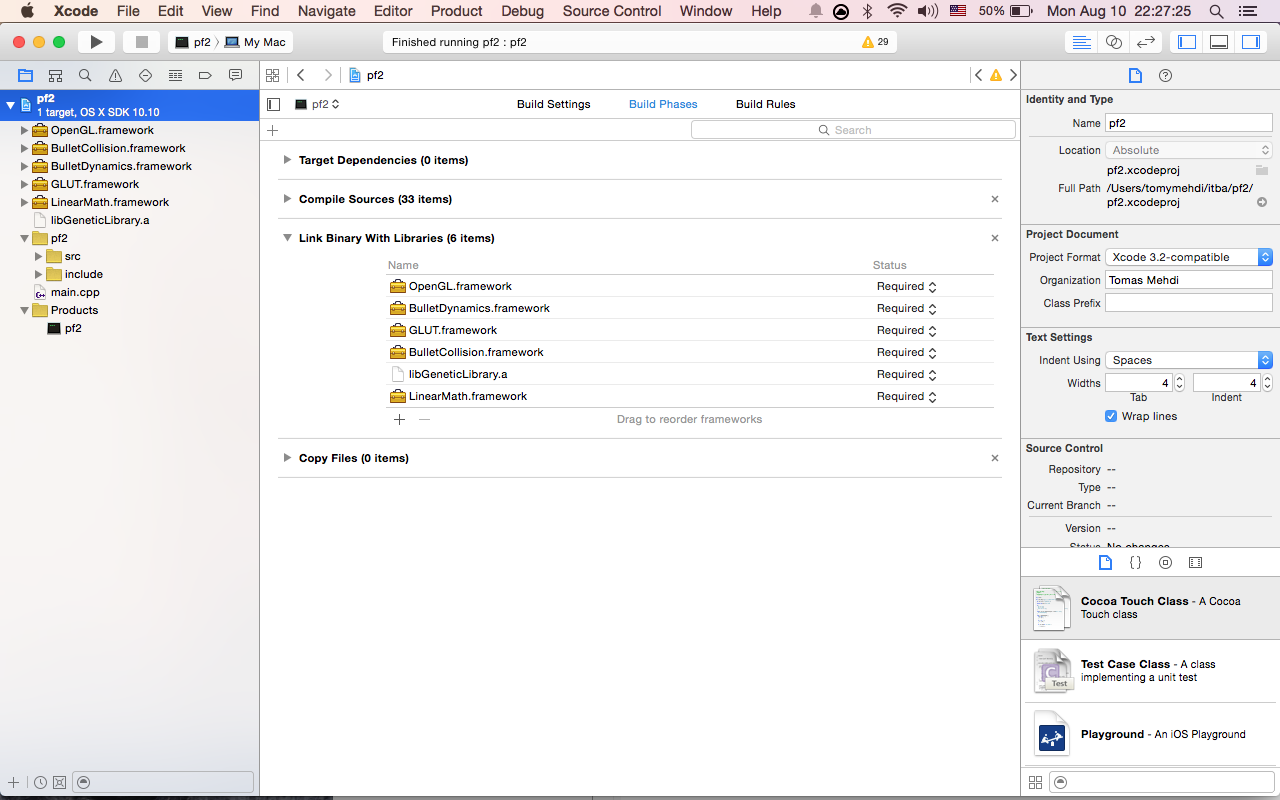
\includegraphics[width=0.72\linewidth]{readme2.png}} 
\end{figure}
%![alt tag](https://raw.githubusercontent.com/ealtamir/pf_experimentos/master/readme1.png)
%![alt tag](https://raw.githubusercontent.com/ealtamir/pf_experimentos/master/readme2.png)

\item Cambiar la ubicaci\'on del $build$ de XCode. Esto es necesario porque en el proyecto se usan paths relativos para leer archivos del directorio del proyecto. Para ello, Ir a las opciones de XCode (shortcut Command-,), luego en el bot\'on Ubicaci\'on > Avanzado, elegir Personalizado y escribir algo como: ``/Users/Username/PF/proyectoDir/bin''; para ``Intermedios'' escribir
 ``/Users/Username/PF/proyectoDir/bin/Intermediates'', donde proyectoDir es el directorio del repositorio de github.
\end{enumerate}


\end{document}
